\documentclass[12pt, letterpaper]{article}
\usepackage[spanish]{babel}
\usepackage[utf8]{inputenc}
\usepackage{graphicx}
\usepackage{amssymb}
\graphicspath{{./imagenes/}}
\usepackage{xcolor}

%Paquetes para símbolos y entornos matematicos. En este documento se usa para poder usar el tag \begin{align} y \begin{align*} que permiten alinear expresiones matemáticas
\usepackage{amsmath}
\usepackage{amssymb}
%paquete que permite el uso de del argumento H al momento de insertar imágenes
\usepackage{float}

%comando para especificar el título del documento 
\title{Matemáticas para las Ciencias Aplicadas I}

%comando para especificar el autor del documento
\author{Pérez Romero Natalia Abigail}

%comando para especificar la fecha del documento
\date{\today}
%--------------Fin preámbulo--------------

%------------Inicio documento-------------
\begin{document}
%comando que genera el titulo con los datos especificados en el preámbulo
\maketitle
\textbf{Tarea XII. Ejercicios del libro Cálculo. Una variable de Thomas J.R, George B.}

\textbf{Ejercicios 13, 19, 36, y 45 de  la sección 2.5 Limites infinitos}

\textbf{13.} Encuentre el límite\\

 $\lim_{ x \to (\pi/2)^-} \tan x  = $\\

$\lim_{ x \to (\pi/2)^-} \tan x  = \lim_{ x \to (\pi/2)^-} \frac{\sen x}{\cos x} =$\\
$\lim_{ x \to (\pi/2)^-} \frac{1}{\cos x} * \sen x = \lim_{ x \to (\pi/2)^-} \frac{1}{\cos \pi/2} * \sen \pi /2 =$\\
$ \lim_{ x \to (\pi/2)^-} \frac{1}{0} * 1 = $ Indeterminación


\begin{figure}[tbh]
\centering
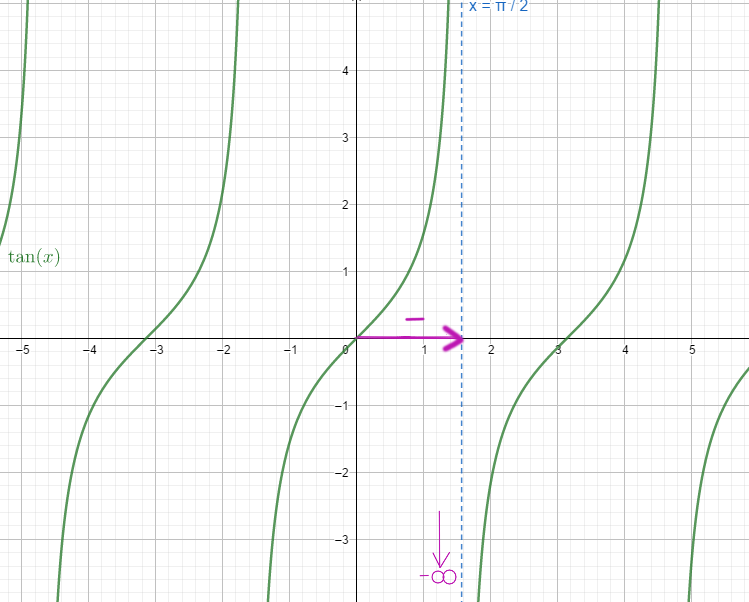
\includegraphics[width=20em]{t12uno}
\end{figure}

$$0 < |x - \frac{\pi}{2}| < \delta => -B$$
$$0 < x - \frac{\pi}{2} < \delta => -B$$
$$ \frac{\pi}{2} < x < \delta + \frac{\pi}{2}  => -B$$

 $\lim_{ x \to (\pi/2)^-} \tan x  = - \infty $\\

\textbf{19.} Encuentre los límites\\
\textbf{a. } $\lim_{ x \to 0^+} (\frac{x^2}{2}-\frac{1}{x}) = \lim_{ x \to 0^+} \frac{x^3-2}{2x}$\\
Recuerdo que para que una función racional este definida en los reales el denominador debe ser distinto de 0 como ya no es posible hacer otra simpificación, entonces $ \lim_{ x \to 0^+} \frac{x^3-2}{2x} = + \infty$\\
y $x= 0$ es una asíntota vertical.\\

\textbf{b. } $\lim_{ x \to 0^-} (\frac{x^2}{2}-\frac{1}{x}) =  -\infty$\\

\textbf{c. } 
$$\lim_{ x \to \sqrt[3]{2}} (\frac{x^2}{2}-\frac{1}{x}) = \lim_{ x \to \sqrt[3]{2}} \frac{x^3-2}{2x} = \\
 \lim_{ x \to \sqrt[3]{2}}  \frac{{(2^{\frac{1}{3}})}^3 -2}{(2^{\frac{1}{3}})} = \lim_{ x \to \sqrt[3]{2}} \frac{2 - 2}{(2^{\frac{1}{3}})} = 0 $$

\textbf{d. } 
$$\lim_{ x \to -1} (\frac{x^2}{2}-\frac{1}{x}) = \lim_{ x \to -1} \frac{x^3-2}{2x} =\lim_{ x \to -1} \frac{(-1)^3-2}{2(-1)} = \lim_{ x \to -1} \frac{-1-2}{-2} =
\frac{3}{2}$$\\

\begin{figure}[tbh]
\centering
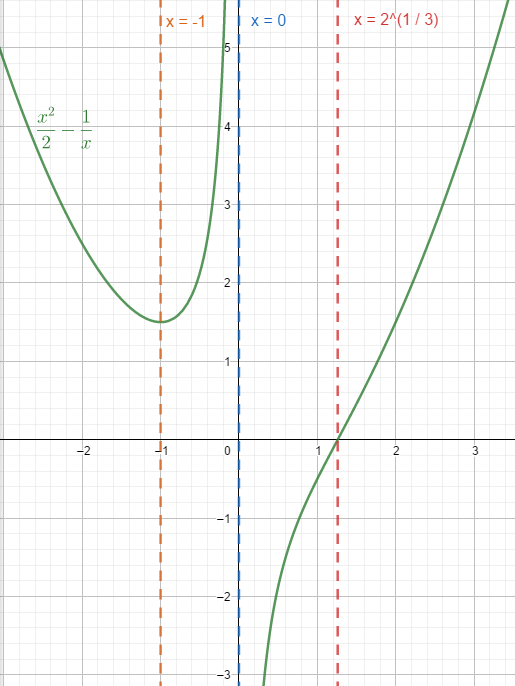
\includegraphics[width=20em]{t12dos}
\end{figure}

\newpage

\textbf{36.} Graficación de funciones racionales\\

 $$y= \frac{x^2 -1}{2x+4}$$
Existe una asíntota vertical en $2x+4= 0 => 2x=4 => x = 2$
No existe una asíntota horizontal , porque el numerador tiene mayor exponente que el denominador.
Asintotas oblicuas $$\frac{x^2-1}{2x+4}= \frac{x}{2}-1$$

\begin{figure}[tbh]
\centering
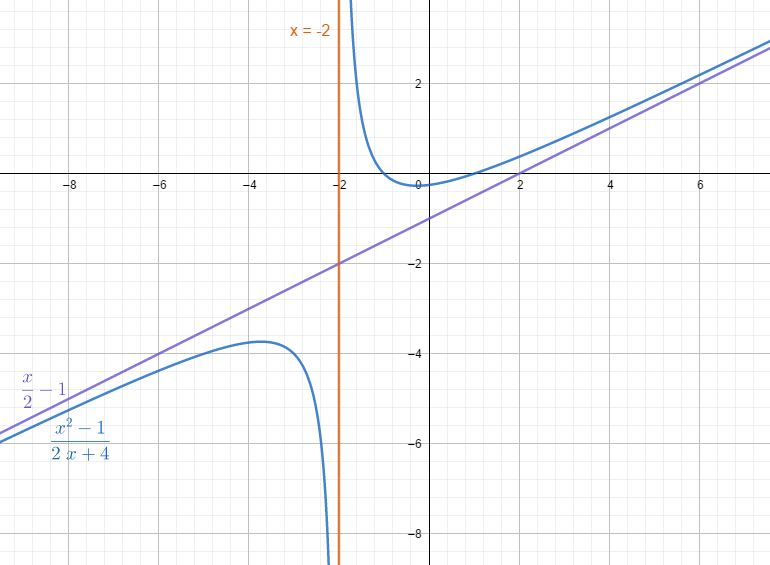
\includegraphics[width=30em]{t12tres}
\end{figure}
\newpage
\textbf{45.} Creación de funciónes\\

\begin{align*}
	\lim_{x \to -\infty} h(x) = -1  \\ 
	\lim_{x \to \infty} h(x) = 1  \\ 
	\lim_{x \to 0^-} h(x) = -1  \\ 
	\lim_{x \to 0^+} h(x) = 1  
\end{align*}


\begin{align*}
f(x)= \left\{ \begin{array}{lcc}
                 (-1 + \frac{1}{x}) &   si  & x \to -\infty \\
	  	\\ (1 + \frac{1}{x}) &   si  & x \to -\infty \\
		\\ (-\frac{3x^2+5x-3}{3x^2+4}) &   si  & x \to 0^- \\
             	\\ (\frac{6x^2-7}{6x^2+11}) &   si  & x \to 0^+
             \end{array}
   \right.
\end{align*}


\end{document} 